\documentclass[11pt]{article}
\usepackage[margin=1in]{geometry}
\usepackage{siunitx}
\usepackage[version=4]{mhchem}
\usepackage{xltabular}
\usepackage{ragged2e}
\usepackage[font=small, skip=3pt, labelfont=bf]{caption}
\usepackage{float}
\usepackage{amsmath}
\usepackage{multirow}
\usepackage{enumitem}
\usepackage{titling}
\usepackage{graphicx}
\usepackage{microtype}
\usepackage[style=apa]{biblatex}

\addbibresource{ia.bib}

\DeclareSIUnit{\mpl}{\mol\per\litre}
\DeclareSIUnit{\mmol}{\milli\mol}
\DeclareSIUnit{\gpm}{\gram\per\mol}
\DeclareSIUnit{\ml}{\milli\litre}

\setlist{nosep}

\sisetup{
	space-before-unit = true,
	free-standing-units = true,
	use-xspace = true
}

\title{The Relationship Between the Time Spent Boiling Tap Water and the Concentration of Dissolved Chlorine in the Water}
\author{jjr117}
\date{}

\begin{document}

\begin{titlingpage}
	\maketitle
\end{titlingpage}

\noindent\textbf{Research Question:} How does the time spent boiling tap water affect the concentration of dissolved chlorine in the water?

\section{Introduction}

Chlorine plays a crucial role in modern water treatment systems. In water treatment facilities, chlorine is added to wastewater to kill deadly bacteria and organisms as part of the water treatment process that converts wastewater into clean drinking water. By the time the treated water arrives at our homes, the chlorine concentration is too low to pose any health risks.

However, while the low concentration of chlorine in tap water makes it safe to consume, it also produces an unpleasant taste. One way my family has been removing the chlorine in tap water is by boiling it before consuming it. However, different sources provide different recommendations on how long water should be boiled for in order to remove chlorine from tap water. Some sources say that 15 minutes is enough to remove all the chlorine from tap water (ESP Water Products), while other sources recommend boiling for at least 20 minutes (Gray 2021). Thus, in my experiment, I plan to investigate the relationship between the time spent boiling tap water and the chlorine concentration remaining in the water. With the data, I hope to determine the optimal amount of time water should be boiled for in order to remove a significant amount of chlorine from the water.

\section{Background Information}

Chlorine gas (\ce{Cl2_{(g)}}) is frequently used at water treatment facilities to remove harmful organisms from wastewater to produce water which is safe for us to consume. When chlorine gas is added to water, the chlorine reacts with water to form hypochlorous acid (\ce{HOCl}):

\centerline{\ce{Cl2_{(g)} + H2O_{(l)} -> HOCl_{(aq)} + H^{+}_{(aq)} + Cl^{-}_{(aq)}}}

Hypochlorous acid is effective at inactivating deadly microbiological organisms like salmonella and E. coli, as well as many viruses (Health Canada 2016). This weak acid is able to kill these harmful organisms by disrupting their cell membranes and destroying their protein structures (Hadhazy 2013). Thus, through the use of chlorine, water treatment facilities are able to remove the harmful bacteria from wastewater that would otherwise cause illness and death.

However, it is not sufficient to add just enough chlorine to disinfect water at the treatment plants. An adequate concentration of chlorine must be sustained throughout the entire distribution system. Otherwise, the water could possibly become infected in intermediate sources and become unsafe to drink by the time it reaches our homes. Because of these concerns, water treatment plants add excess chlorine to treat water such that the water that comes out of our faucets still contains a small concentration of free chlorine—chlorine that has not yet reacted with undesired substances in the water.

The free chlorine in tap water is what gives it an unpleasant taste, even in low concentrations. To remove this excess chlorine, my family boils tap water for around 15 to 20 minutes. Boiling is effective at removing chlorine because the solubility of gases in liquids decreases as the temperature of the liquid increases, and chlorine is a gas at room temperature. Thus, as the water is heated up, it cannot hold as much dissolved free chlorine in the water, and so some of the free chlorine is released from the water in the form of chlorine gas.

\begin{figure}[H]
	\centering
	\caption{Solubility curve for chlorine: the hotter the water is, the less dissolved chlorine the water can hold.}
	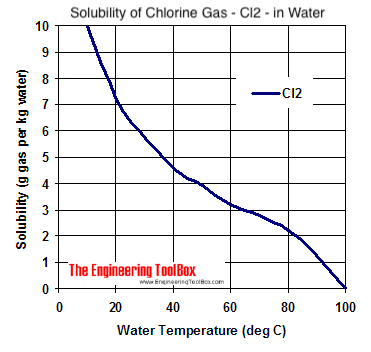
\includegraphics[width=0.5\linewidth]{assets/cl-solubility.png}
\end{figure}

In addition to investigating the relationship between boiling water and the remaining chlorine concentration, I hope to compare the effectiveness of boiling water with another method of removing chlorine from water: water deionizers.

Water deionizers remove chlorine through ion-exchange resins. One resin contains beads which are positively pre-charged with hydrogen ions (\ce{H^+}), and the other resin contains beads which are negatively pre-charged with hydroxide ions (\ce{OH^-}). Water contaminated with minerals is passed through both resins in the water deionizer. The positively changed resin exchanges its hydrogen ions with cations present in the water, and the negatively changed resin exchanges its hydroxide ions with anions present in the water, such as chloride ions. In the end, the hydrogen ions and hydroxide ions combine to form pure water \ce{H2O} (Olszak 2020).

\subsection{Hypothesis}
I hypothesize that the time spent boiling tap water is inversely proportional to the concentration of dissolved chlorine in the water. In addition, I hypothesize that the water deionizer will be more effective at removing chlorine compared to boiling water for less than 15 minutes. But, when the water is boiled for around 15-20 minutes, I predict that the concentration of chlorine from the water deionizer will be similar to that of the boiled water.

\section{Methodology}

To determine the amount of chlorine in a sample of tap water, Mohr's method was used. Mohr's method determines the chloride ion concentration in a solution (the analyte) by titrating it with silver nitrate (\ce{AgNO3}) and adding potassium chromate (\ce{K2CrO4}) as an indicator.

Initially, the analyte consists of the water sample and a few drops of the potassium chromate indicator, which turns the analyte light yellow:

\begin{figure}[H]
	\centering
	\includegraphics[width=0.25\linewidth]{assets/initial.png}
	\caption{Before any silver nitrate solution is added, the colour of the solution is a bright and transparent yellow.}
\end{figure}

As the silver nitrate solution from the burette is slowly added to the analyte, the chloride ions in the analyte bond with the silver ions to form silver chloride:

\centerline{\ce{Ag^{+}_{(aq)} + Cl^{-}_{(aq)} -> AgCl_{(s)}}}

Since silver chloride is insoluble in water, it produces a white precipitate that can be seen after the titration starts but before the endpoint is reached:

\begin{figure}[H]
	\centering
	\includegraphics[width=0.25\linewidth]{assets/white-precipitate.png}
	\caption{The silver chloride is visible as an insoluble white precipitate.}
\end{figure}

Then, once the silver ions have reacted with all the chloride ions in the analyte, the silver ions will then start reacting with the chromate ions from the potassium chromate indicator to form silver chromate (\ce{Ag2CrO4_{(s)}}):

\centerline{\ce{2Ag^{+}_{(aq)} + CrO4^{2-}_{(aq)} -> Ag2CrO4_{(s)}}}

Silver chromate is an insoluble red-brown precipitate. Its presence can be easily identified in the analyte as it causes the colour of the solution to change from white to a red-brown colour:

\begin{figure}[H]
	\centering
	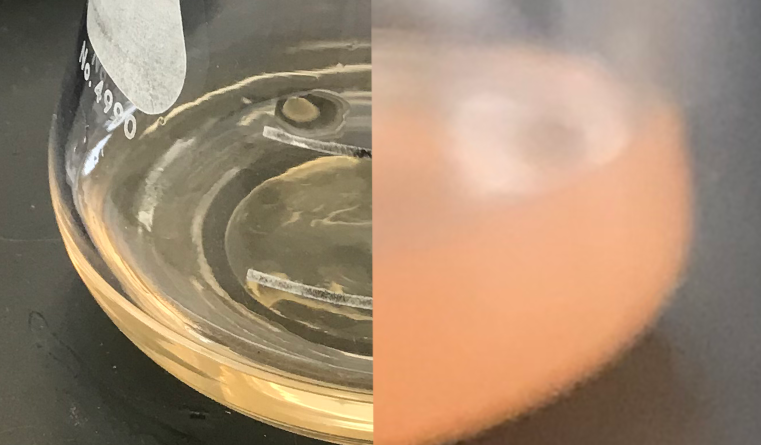
\includegraphics[width=0.3\linewidth]{assets/color-difference}
	\caption{The color difference between the starting point of the titration (left image) and the endpoint of the titration (right image).}
\end{figure}

The titration stops when the red-brown colour appears throughout the solution, even after vigorous shaking. This indicates that all the chloride ions have reacted and that the endpoint has been reached. The amount of the silver nitrate solution titrant added to the analyte is then noted down. This amount can be used to determine the amount of chloride ions that is present in the water sample.

One potential weakness with Mohr's method is that it is ineffective at determining the chlorine concentration of a water sample containing other halides, such as iodide or bromide. However, Toronto's tap water is regulated to contain a maximum of \SI{0.01}{\milli\gram\per\litre} of bromate in tap water (Health Canada, 2015), which is 100 times less than the concentration of chlorine in tap water. The concentration of iodide in tap water is also extremely trace at around \SI{4}{\micro\gram\per\litre} (World Health Organization, 1996). Thus, the bromide concentration and iodide concentration in tap water is relatively negligible and will not significantly affect the results obtained using Mohr's Method to determine the chlorine concentration.

\subsection{Variables}

\textbf{Independent Variable:} Amount of time spent boiling tap water

\smallskip

\noindent\textbf{Dependent Variable:} Chlorine concentration in the boiled tap water

\begin{table}[H]
	\def\arraystretch{1.5}
	\caption{A list of controlled variables during the experiment.}
	\begin{tabularx}{\linewidth}{|
			>{\RaggedRight}X|
			>{\RaggedRight}X|
			>{\RaggedRight}X|
		}
		\hline
		\textbf{Controlled Variable}
		 & \textbf{Reason for Control}
		 & \textbf{Method of Control}
		\\\hline
		Temperature of the hot plate
		 & Different temperatures of the hot plate would boil water at different speeds.
		 & The hot plate was initially left on for 15 minutes to reach full power. Then, the water samples were boiled sequentially with the hot plate continuously on at full temperature when boiling each of the samples.
		\\\hline
		Amount of water added to each sample
		 & The visibility of the endpoint is affected by the volume of water (more water makes the red-brown colour at the titration endpoint more diluted and less visible).
		 & A 10\ml sample of the boiled tap water was used for each trial.
		\\\hline
	\end{tabularx}
\end{table}

\newpage

\subsection{Apparatus}

\begin{itemize}
	\item 25\ml graduated cylinder with 1\ml graduations
	\item 100\ml graduated cylinder with 1\ml graduations
	\item Analytical scale with $\pm$0.0001\gram precision

	\item Hot Plate
	\item 50\ml Burette with 0.1\ml graduations
	\item Burette stand
	\item Funnel

	\item 5 $\times$ 250\ml Glass Beaker
	\item 250\ml Erlenmeyer Flask
	\item 10\ml pipette

	\item Water deionizer (Thermo Scientific HN High Capacity Cartridge)

	\item 2 $\times$ 1\litre Glass Beaker
	\item 1\ml Droppers
	\item Scoopula
\end{itemize}

\subsection{Materials}

\begin{itemize}
	\item Silver Nitrate (\ce{AgNO3_{(s)}}, powdered form)
	\item 0.1 \mpl Potassium Chromate Solution (\ce{K2CrO4_{(aq)}})
	\item Deionized Water
\end{itemize}

\subsection{Risk Assessment}

Even though chlorine gas is released when tap water is boiled, the amount of chlorine released is so trace that it poses no appreciable danger. According to the City of Toronto's website, the amount of chlorine in drinking water is regulated to be between 1 and \SI{3}{\mg\per\litre}, which is equal to 1-3 ppm. At this concentration of chlorine gas, mild mucus membrane irritation occurs that can be tolerated for around an hour (National Library of Medicine, 2010). However, because the experiment is conducted in a large and ventilated room and the chlorine gas from boiling tap water is released over a relatively long period of time, the actual concentration of the chlorine gas at any given moment is much lower, thus posing no threat as a health hazard.

Silver nitrate, however, is hazardous and can stain skin and cause damage if it comes in contact with the eyes (New Jersey Department of Health, 2009). Thus, goggles were worn at all times during the experiment and gloves were worn when handling silver nitrate. In addition, silver nitrate is considered hazardous waste due to its reactivity and toxicity, so it must be disposed properly. After each trial, the solution containing tap water, silver nitrate solution and potassium chromate solution was poured into a temporary 1\litre beaker for storing waste. Once all the experiments were finished, the remaining silver nitrate solution in the burette and the contents of the waste beaker were poured in a hazardous waste container provided by the school.

In addition, this experiment involves boiling water with the use of a hot plate at maximum power. Thus, it was crucial that the hot plate was placed away from the main titration setup to prevent accidental contact. In addition, gloves were worn when the beakers needed to be placed on and removed from the hot plate to prevent burns. When the beakers were removed from the hot plate, they were placed in a large 1\litre beaker containing around 100\ml of cold water. This minimized the risk of spilling the hot water and causing damage. Cooling down the water before titration should not affect the end result, as the purpose of boiling the water is to remove free chlorine dissolved in the water. By the time the water is cooled, the free chlorine should have been already released into the atmosphere as chlorine gas, after which it will not become re-dissolved in the water.

\subsection{Preparation}

A dilute solution of 0.01\mpl \ce{K2CrO4_{(aq)}} was created by measuring out 2\ml of the 0.1\mpl \ce{K2CrO4_{(aq)}} stock solution and diluting it with 20\ml of deionized water in a 25\ml graduated cylinder. Optimally, a more concentrated potassium chromate solution would have been created, but this was not feasible due to supply limitations.

To create the silver nitrate solution (\ce{AgNO3_{(aq)}}), 0.0817\gram of solid \ce{AgNO3} using a scoopula and an analytical scale. The silver nitrate was then dissolved in 50\ml of deionized water measured using a 100\ml graduated cylinder. The concentration of this solution was designed to equal approximately 0.01\mpl.

\section{Procedure}

\begin{enumerate}
	\item The hot plate was turned on and set to max power. It was left to heat up for around 15 minutes in order to reach max temperature.

	\item The 50\ml silver nitrate solution was poured into the burette using a funnel, and the burette was secured onto the burette stand.

	\item The 1\litre beaker was filled with around 100\ml of cold water.

	\item Five 250\ml glass beakers were filled with 100\ml tap water each. Tape was used to label the beakers with 0, 3, 6, 9, and 20 minutes of boiling.

	\item Once the hot plate had reached max temperature, the tape on the 250\ml beaker labeled with 3 minutes was removed and placed on the desk beside the hot plate. Then, gloves were worn and the beaker was placed onto the hot plate.

	\item A timer was prepared, and the water in the beaker was observed. The timer was started when the large bubbles consistently rose to the surface of the water, indicating that it was boiling. Once the timer reached 3 minutes, gloves were used to remove the beaker from the hot plate. The beaker was then placed in the 1\litre beaker with cold water to cool down. The tape was then placed next to the cold water beaker.

	\item Steps 5-6 were repeated for the beakers labeled with 6, 9, and 20 minutes. Once the timer was one minute away, the beaker in the cold water was removed. The corresponding label was also re-placed on the removed beaker.

	\item 10\ml of tap water from the beaker labeled ``0 minutes'' was transported into a 100\ml Erlenmeyer flask using a 10\ml pipette.

	\item 1\ml of the 0.01\mpl \ce{K2CrO4} solution was added to the 100\ml Erlenmeyer flask using a 1\ml dropper.

	\item The initial volume of \ce{AgNO3} solution in the burette was noted down. The tap water in the Erlenmeyer flask was titrated with the \ce{AgNO3} solution until the solution turned red-brown and remained red-brown even after vigorous shaking (see Figure 4). Then, the titration is stopped and the final amount of \ce{AgNO3} solution in the burette was noted down.

	\item The solution in the Erlenmeyer flask was poured into the 1\litre beaker for temporarily holding the waste products from the titration. The flask was then rinsed with deionized water, and steps 8-11 were repeated for 2-3 more trials.

	\item Steps 8-11 were then repeated for the beakers labeled with 3, 6, 9, and 20 minutes and also repeated for deionized water.
\end{enumerate}

\section{Data}

% \begin{noindent}
<?
const silverNitrateSol = {
	mass: 0.0817,
	volume: 0.05,
	concentration: undefined,
};

/*
[0]: # of minutes boiled (or 'deionized' if the water was deionized)
[1]: mL of AgNO3 needed
[2]: mL of H2O used
*/

const rawData = [
	['deionized', 11.75 - 11.45, 10],
	['deionized', 31.15 - 30.8, 10],
	['deionized', 31.6 - 31.15, 10],
	[0, 11.45 - 10.15, 10],
	[0, 17.45 - 16.2, 10],
	[0, 18.7 - 17.45, 10],
	[3, 5.6 - 4.3, 10],
	[3, 14.3 - 13, 10],
	[3, 13 - 11.75, 10],
	[6, 20.15 - 18.7, 10],
	[6, 30.8 - 29.4, 10],
	[6, 7 - 5.6, 10],
	[9, 16.2 - 14.3, 10],
	[9, 10.15 - 8.65, 10],
	[20, 26.4 - 20.15, 10],
	[20, 29.4 - 23.4, 10],
];

const headers = ['minutesBoiled', 'titrantAmount', 'amountOfWater'];

const data = rawData.map(row => Object.fromEntries(R.zip(headers, row)));
?>
% \end{noindent}

\begin{table}[H]
	\caption{Data collected during the experiment over 16 trials. The amount of water titrated for each trial was 10\ml $\pm$ 0.05\ml .}
	\def\arraystretch{1.2}
	\begin{tabularx}{\linewidth}{|
			>{\RaggedRight}X|
			>{\RaggedRight}X|
			>{\RaggedRight}X|
			>{\RaggedRight}X|
		}
		\hline
		\textbf{Trial Number}              &
		\textbf{Time Boiled} /\si{\minute} &
		\textbf{Titrant Amount} /$\pm$0.1\ml
		\\\hline
		% \begin{noindent}
		<? for (const [rowIndex, row] of data.entries()) { ?>
			Trial <?= rowIndex + 1 ?>
			& <?= row.minutesBoiled ?>
			& <?= row.titrantAmount.toFixed(2) ?>
			\\\hline
		<? } ?>
		% \end{noindent}
	\end{tabularx}
\end{table}

\section{Calculations}

To determine the concentration of chloride ions in the water, the amount of water and the amount of titrant is used.

The mass of \ce{AgNO3_{(s)}} used to create the silver nitrate solution was <?= silverNitrateSol.mass ?>\g. The analytical scale used to weigh this amount had an uncertainty of $\pm$0.0001\g. Using this information, the number of moles of silver nitrate in the solution can be determined:
%
\begin{align*}
	n_{\ce{AgNO3}} & = \frac{m_{\ce{AgNO3}}}{M_{\ce{AgNO3}}}
	\\
	n_{\ce{AgNO3}} & = \frac{(<?= silverNitrateSol.mass ?> \pm 0.0001)\g}{169.87\gpm}
	\\
	<? silverNitrateSol.moles = silverNitrateSol.mass / 169.87 -?>
	n_{\ce{AgNO3}} & = <?= sf(silverNitrateSol.moles, 3) ?>\mol \pm <?= sf(0.0001 / silverNitrateSol.mass * 100, 1) ?>\%
\end{align*}

The silver nitrate was diluted with 50\ml of deionized water using a graduated cylinder with an uncertainty of 0.5\ml or 1\%. Using the number of moles of \ce{AgNO3} in the solution, the concentration of the solution can be determined:
%
\begin{align*}
	c & = \frac{n}{V}
	\\
	c & = \frac{<?= sf(silverNitrateSol.moles, 3) ?>\mol \pm 0.1\%}{<?= silverNitrateSol.volume ?>\litre \pm 1\%}
	\\
	<? silverNitrateSol.concentration = silverNitrateSol.moles / silverNitrateSol.volume -?>
	c & = <?= sf(silverNitrateSol.concentration, 3) ?>\mpl \pm 1.1\%
\end{align*}

The concentration of the \ce{AgNO3} solution can then be used to determine the moles of \ce{AgNO3} for a given volume of the silver nitrate solution. For example, using the data in Trial 4, the volume of the silver nitrate solution needed to titrate the water was 1.30\ml $\pm$ 0.1\ml, or 1.30\ml $\pm$ 7.7\%, giving the following number of moles of \ce{AgNO3}:
%
\begin{align*}
	n & = V \times c
	\\
	n & = (1.30\ml \pm 7.7\%) \times (<?= sf(silverNitrateSol.concentration, 3) ?>\mpl \pm 1.1\%)
	\\
	<? const trial1Calculations = { molesOfSilverNitrate: silverNitrateSol.concentration * 1.30 } -?>
	n & = <?= sf(trial1Calculations.molesOfSilverNitrate, 3) ?>\mmol \pm 8.8\%
\end{align*}

The number of moles of \ce{AgNO3} can then be used to determine the number of moles of chloride ions in the water. The mole ratio between \ce{Ag^-} and \ce{Cl^-} can be determined from the reaction taking place between the silver nitrate and the chloride ions:

\centerline{\ce{AgNO3_{(aq)} + Cl^{-}_{(aq)} -> AgCl_{(s)} + NO3^{-}_{(aq)}}}

From the above balanced chemical equation, it can be determined that the mole ratio between \ce{Ag^-} and \ce{Cl^-} is 1. Therefore, the number of moles of \ce{AgNO3} is equal to the number of moles of \ce{Cl^-}:
%
\begin{align*}
	n_{\ce{Cl^-}} & = n_{\ce{AgNO3}}
	\\
	<? trial1Calculations.molesOfChlorine = trial1Calculations.molesOfSilverNitrate -?>
	n_{\ce{Cl^-}} & = <?= sf(trial1Calculations.molesOfChlorine, 3) ?>\mmol \pm 8.8\%
\end{align*}

From here, the concentration of chloride ions in the water can be determined knowing that the amount of water used was 10\ml $\pm$ 0.05\ml, or 10\ml $\pm$ 0.5\%:
%
\begin{align*}
	c & = \frac{<?= sf(trial1Calculations.molesOfChlorine, 3) ?>\mmol \pm 8.8\%}{10\mL \pm 0.5\%}
	\\
	c & = <?= sf(trial1Calculations.molesOfChlorine / 10, 3) ?>\mpl \pm 9\%
\end{align*}

The above calculations were performed for each of the values in the 16 trials, producing the following values:

% \begin{noindent}
<?
function calculateMolesOfChlorine(rowIndex: number) {
	const row = data[rowIndex];
	return row.titrantAmount * silverNitrateSol.concentration / row.amountOfWater;
}

function calculateMolesOfChlorineUncertaintyPercentage(rowIndex: number) {
	const row = data[rowIndex];
	const silverNitrateUncertaintyPercentage = 1.1;
	const titrantUncertaintyPercentage = (0.1 / row.titrantAmount) * 100;
	const amountOfWaterUncertaintyPercentage = 0.5;
	const totalUncertaintyPercentage =
		silverNitrateUncertaintyPercentage +
		titrantUncertaintyPercentage +
		amountOfWaterUncertaintyPercentage;
	return totalUncertaintyPercentage;
}

function formatFinalMolesOfChlorine(rowIndex: number) {
	const moles = calculateMolesOfChlorine(rowIndex);
	const uncertaintyPercentage = calculateMolesOfChlorineUncertaintyPercentage(rowIndex);
	return roundToUncertaintyDecimalPlaces(moles, uncertaintyPercentage);
}

function roundToUncertaintyDecimalPlaces(value: number, uncertaintyPercentage: number) {
	const uncertaintyString = sf(value * (uncertaintyPercentage / 100), 1);
	const decimalPlaces = uncertaintyString.length - uncertaintyString.indexOf('.') - 1;
	return `${value.toFixed(decimalPlaces)} $\\pm$ ${uncertaintyString}`;
}
?>
% \end{noindent}

\begin{table}[H]
	\caption{The concentration of chloride ions in each trial obtained from performing the above calculations. For each variation of boiling time, the uncertainty in the average concentration of \ce{Cl^-} was determined by taking the average of the uncertainties for each individual trial.}
	\def\arraystretch{1.5}
	\begin{tabularx}{\linewidth}{|
			>{\RaggedRight}X|
			>{\RaggedRight}X|
			>{\RaggedRight}X|
		}
		\hline
		\textbf{Time Boiled} /\si{\minute}
		 & \textbf{Concentration of \ce{Cl^-}} /\si{\mpl}
		 & \textbf{Average concentration of \ce{Cl^-}} /\si{\mpl}
		\\\hline
		% \begin{noindent}
		<? for (const [rowIndex, row] of data.entries()) { ?>
			<?= row.minutesBoiled ?>
			& <?= formatFinalMolesOfChlorine(rowIndex) ?>
			&
			<? if (row.minutesBoiled !== data[rowIndex - 1]?.minutesBoiled) { ?>
				<?
					const end = data.findIndex((dataRow, i) => i >= rowIndex && dataRow.minutesBoiled !== row.minutesBoiled);
					const trialIndexes = R.range(rowIndex, end === -1 ? data.length : end);
					const trialMoles = trialIndexes.map(
						(trialIndex) => calculateMolesOfChlorine(trialIndex)
					);
					const averageMolesOfChlorine = R.mean(trialMoles);
					const sumOfUncertaintyOfAverage = R.sum(trialIndexes.map(
						(trialIndex) =>
							calculateMolesOfChlorine(trialIndex) *
							(calculateMolesOfChlorineUncertaintyPercentage(trialIndex) / 100)
					));
					const uncertaintyPercentageOfAverage =
						sumOfUncertaintyOfAverage / R.sum(trialMoles) * 100
				?>
				\multirow{
					<?=
						R.count(
							(r) => r.minutesBoiled === row.minutesBoiled,
							data
						)
					?>
				}{*}{<?= roundToUncertaintyDecimalPlaces(averageMolesOfChlorine, uncertaintyPercentageOfAverage) ?>}
				\\\cline{1-2}
				<? console.log(row, averageMolesOfChlorine) ?>
			<? } else if (row.minutesBoiled !== data[rowIndex + 1]?.minutesBoiled) { ?>
				\\\hline
			<? } else { ?>
				\\\cline{1-2}
			<? } ?>
		<? } ?>
		% \end{noindent}
	\end{tabularx}
\end{table}

\newpage

Plotting these values on a graph yields the following result:

\begin{figure}[H]
	\centering
	\caption{The concentration of chlorine remaining plotted against boiling time. The orange line represents the average chlorine concentration in the trials that used deionized water.}
	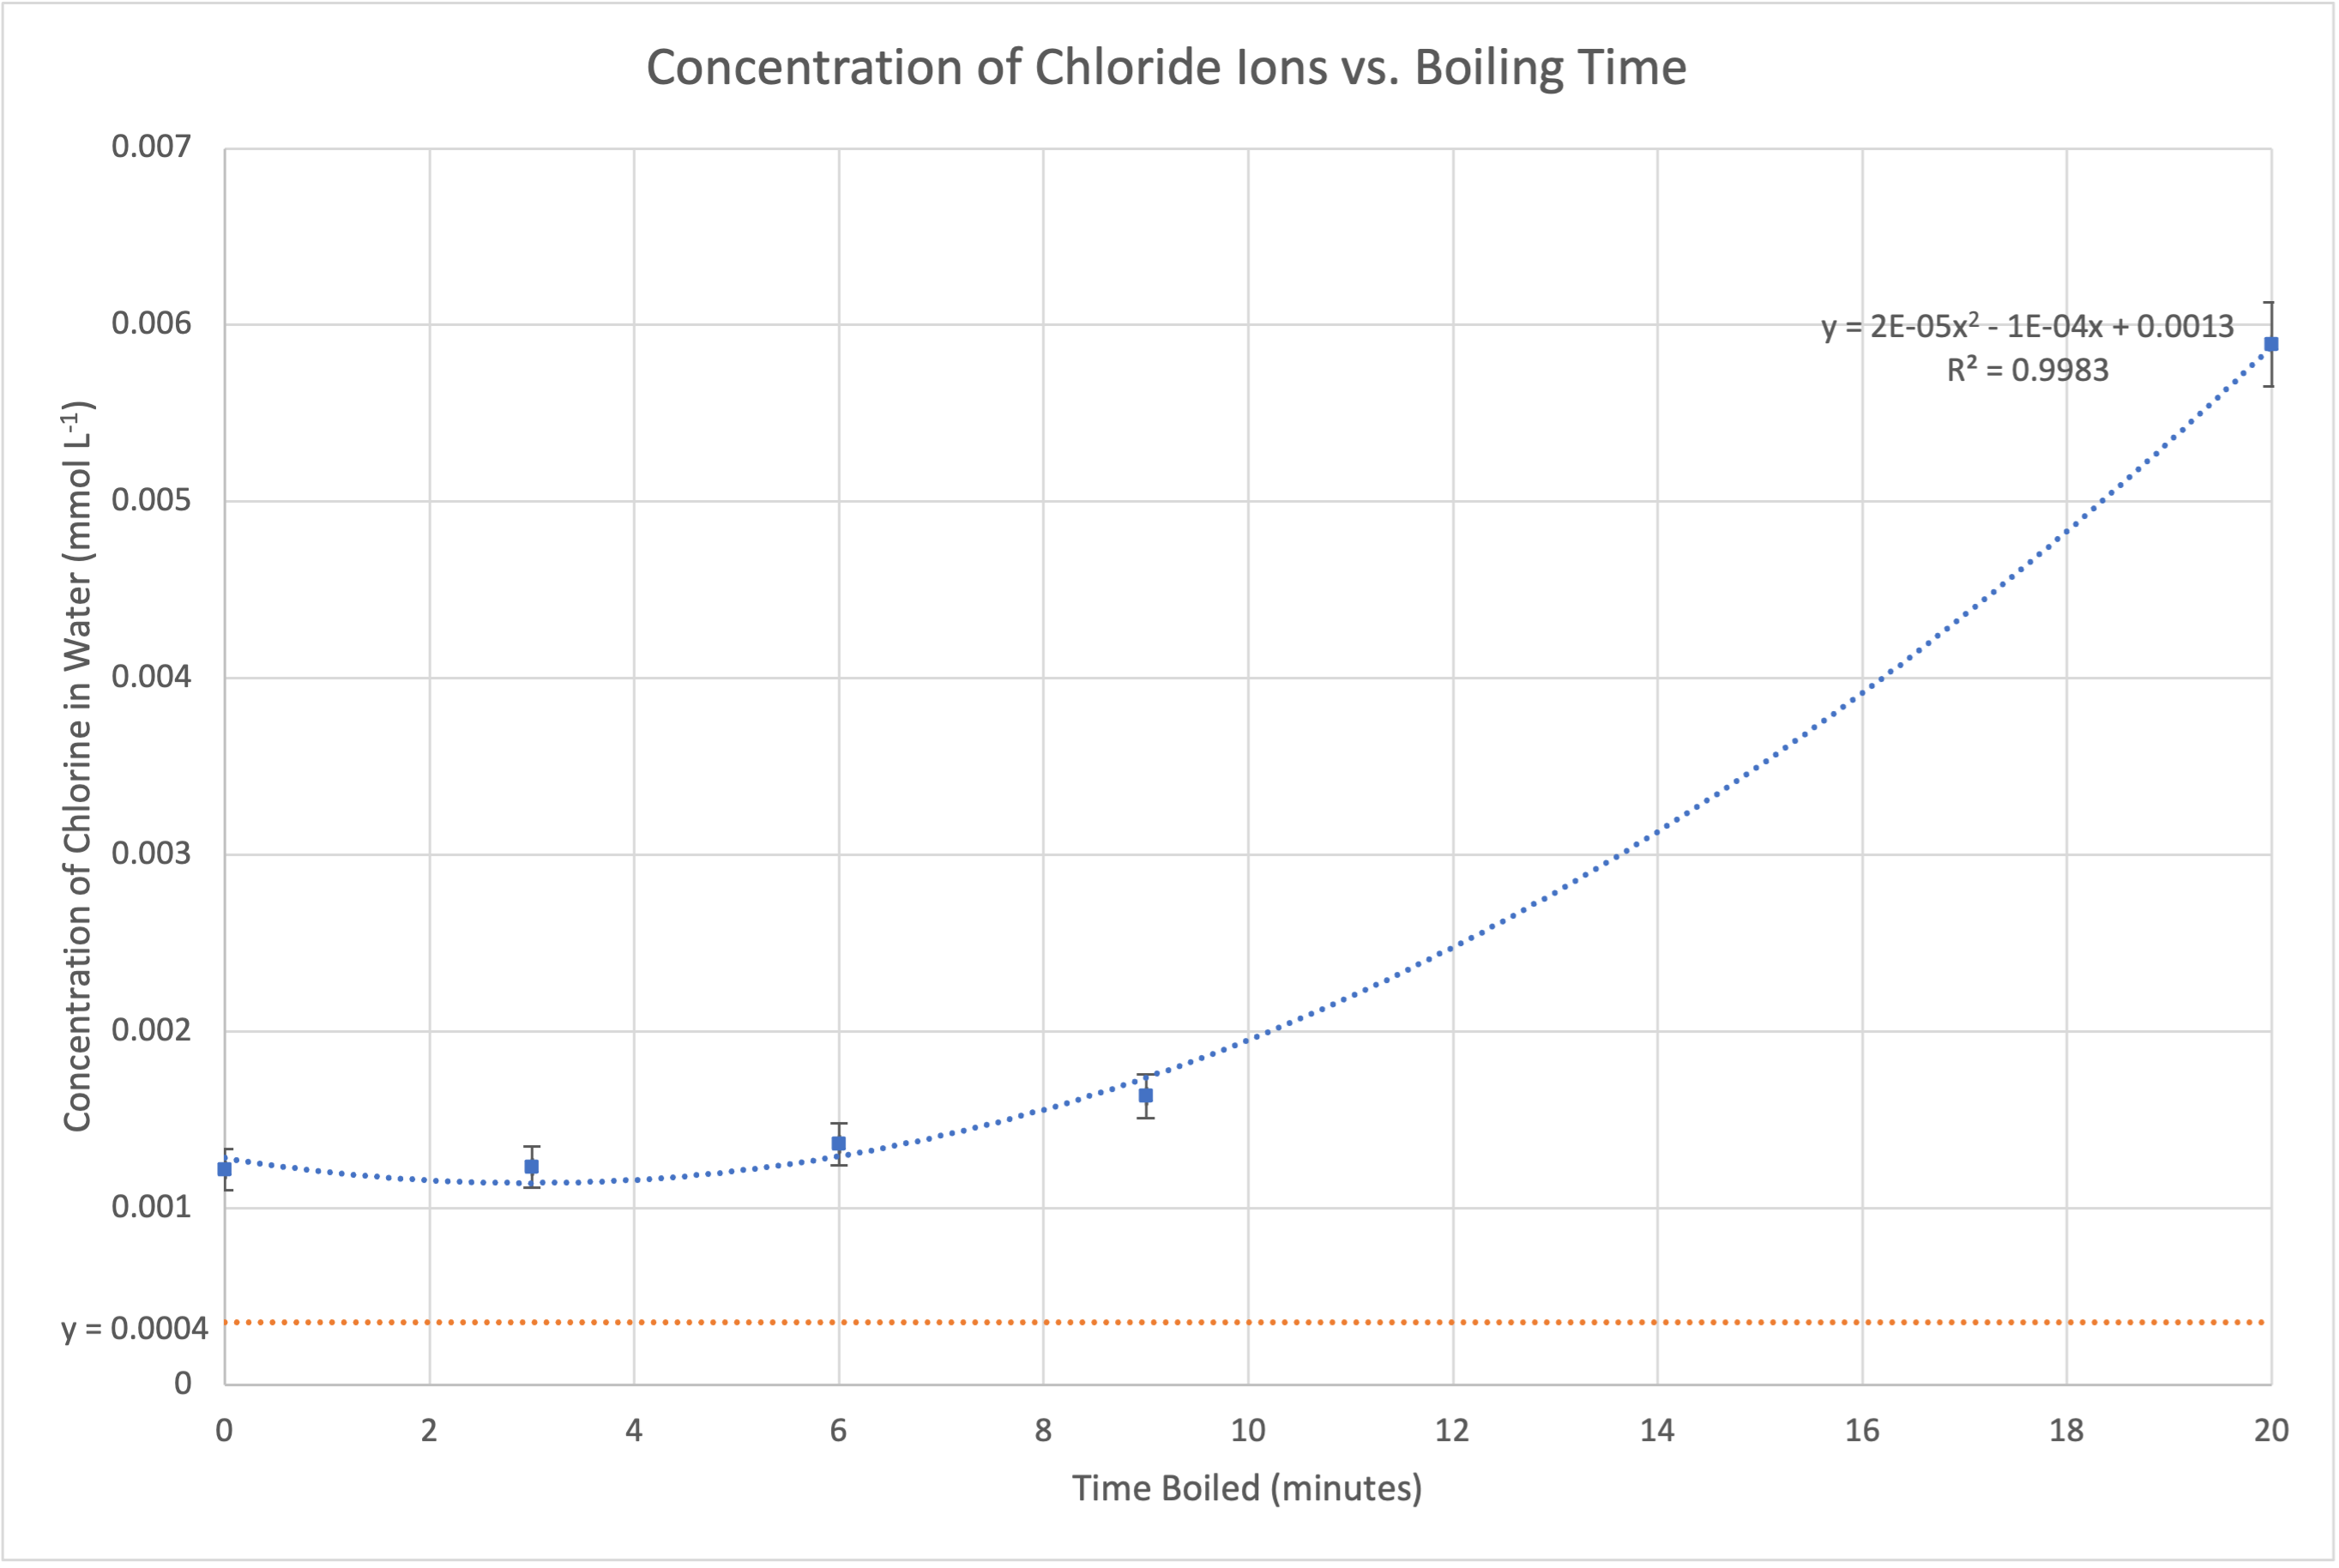
\includegraphics[width=\linewidth]{assets/concentration-vs-boiling-time.png}
\end{figure}

\section{Analysis}

\subsection{Identifying the Correlation}

The equation of the trendline can be written as follows, where $t$ represents the time the water has been boiled (in minutes) and $y$ represents the concentration of chloride in the water (in \si{\mmol\per\litre}):
%
\begin{align*}
	y = 0.00002t^2 - 0.001t + 0.0013
\end{align*}

This equation indicates that there is a positive quadratic relationship between boiling time and chlorine concentration. This relationship does not agree with the hypothesis presented earlier, where it was predicted that the chlorine concentration in the water would \textit{decrease} as the water was boiled for longer. Instead, the graph indicates that the chlorine concentration \textit{increases} as the water was boiled for longer.

\subsection{Interpreting the Results}

The hypothesis was made under the belief that Toronto used only chlorine for water treatment. However, upon further research, it was discovered that there was a misunderstanding and that Toronto also adds ammonia during wastewater treatment.

This detail is significant because when ammonia is added to chlorine, it forms chloramine (\ce{NH2Cl}), which is more stable compared to dissolved chlorine because of the bond between chlorine and ammonia. This stability allows chloramine to remain in the water supply for a longer period of time to ensure that the water remains disinfected for longer. However, the extra stability of chloramine also makes boiling water an ineffective way to remove chloramine from water. Unlike chlorine, it can take hours to boil off an appreciable amount of chloramine from tap water (Byrd 2022).

Thus, the positive correlation depicted in the data between the time spent boiling water and the chlorine concentration in the water strongly suggests that the tap water used in the experiment was treated with chloramine. This conclusion is further supported by the effectiveness of the deionizer used in trials 1 to 3—the concentration of chlorine in the deionized water was significantly lower than the concentration of chlorine in unboiled tap water. Unlike boiling, the water deionizer is effective at removing chloramine, which is dissolved in water as positively charged ammonia ions and negatively charged chloride ions. The positively charged resin in the water deionizer filters out the ammonia ions, and the negatively charged resin in the water deionizer filters out chloride ions. Thus, the water deionizer is still able to produce water which is relatively free of dissolved chlorine even when the water contains chloramine.

The positive correlation between the time spent boiling water and the concentration of dissolved chlorine can be attributed to the decrease in the volume of water. Since boiling water for 20 minutes or less does not release a substantial amount of chloramine, the amount of chloramine is around the same in the water samples in each 100\ml beaker after boiling. However, as the water is boiled for longer, the volume of water decreases as more water evaporates from the beaker. Since the concentration is inversely proportional to the volume of the solution, as the volume of water decreases and the amount of chloramine is held constant, the concentration of chloramine in the water increases. This explains why the chlorine concentration seems to increase as the water is boiled for longer.

The quadratic nature of the relationship is likely explained by the increasing rate of evaporation as the water is boiled. As the water evaporates, the volume of water in the beaker decreases, which in turn causes the energy transferred from the hot plate to heat up the remaining amount of water more quickly. This then increases the rate of evaporation, explaining the quadratic relationship between the time spent boiling water and the volume of water remaining. Since the concentration of chloramine is inversely proportional to the remaining volume of water, the relationship between the concentration of chlorine in the water and the time spent boiling the water must also be a quadratic relationship.

\subsection{Comparison with Expected Value}

The accuracy of the titration can be determined by comparing the experimental results of the chlorine concentration in unaltered tap water with the expected chlorine concentration in tap water regulated by the city of Toronto (between 1\mg/\litre and 3\mg/litre). In order to compare the experimental data with this value, the concentration of chlorine in \si{\mpl} must be converted to \si{\mg\per\litre}:
%
\begin{align*}
	m_{\ce{Cl^-}} & = n_{\ce{Cl^-}} \times M_{\ce{Cl^-}}
	\\
	M_{\ce{Cl^-}} & = 35.45\gpm
	\\
	m_{\ce{Cl^-}} & = (<?= sf(trial1Calculations.molesOfChlorine, 3) ?> \pm 8.8\% \mmol) \times 35.45\gpm
	\\
	<? trial1Calculations.massOfChlorine = trial1Calculations.molesOfSilverNitrate * 35.45 -?>
	m_{\ce{Cl^-}} & = <?= sf(trial1Calculations.massOfChlorine, 3) ?>\mg
	\\
	c             & = <?= sf(trial1Calculations.massOfChlorine, 3) ?>\mg/10\ml
	\\
	c             & = <?= sf(trial1Calculations.massOfChlorine * 100, 3) ?>\mg/\litre
\end{align*}

Surprisingly, compared to the expected value of 1 to \SI{3}{\mg\per\litre}, this result is off by an order of magnitude. The experimental results indicate that there is over 10 times the amount of chlorine that is expected from Toronto's tap water. It is very unlikely that this result represents the actual concentration of Toronto's tap water but rather represents potential sources of error in the titration procedure.

\subsection{Potential Sources of Error}

The discrepancy between the experimental data and the expected data may be attributed to the dilute solutions of silver nitrate and potassium chromate used in the experiment. Due to availability limitations, the concentration of potassium chromate needed to be scaled down to 0.01\mpl compared to the recommend amount of 0.25\mpl to perform Mohr's titration. In addition, the concentration of silver nitrate solution needed to be scaled down to 0.01\mpl as well in order to gain more precision since the amount of tap water in chlorine is very trace. Thus, it is likely that the initial visual colour change was too faint to notice, and an excess of silver nitrate was needed in order to produce a visible colour change that indicated the titration's endpoint. However, this discrepancy would represent a systematic error in the experiment, and thus does not invalidate the positive correlation between the boiling time and the remaining chlorine concentration in water.

\section{Conclusion}

The original purpose of the experiment was to find the relationship between time spent boiling tap water and the remaining concentration of dissolved chlorine assuming the chlorine was present as dissolved chlorine gas. Instead, the data collected from the experiment strongly suggested that the chlorine used to disinfect Toronto's drinking water is not just chlorine gas, but instead dissolved chloramine. However, despite this misunderstanding, the experiment still displayed an evident trend that proved fruitful for analysis. While the data cannot make any conclusions about the effectiveness of boiling water with dissolved chlorine gas, it does conclude that boiling water is not an effective means of removing chloramines from water. Thus, instead of boiling water, my family should consider investing in more efficient methods of water purification which remove chloramine more effectively, such as a carbon block filter or a reverse osmosis filter.

Despite the inaccuracy between the experimental value and expected value of chlorine concentration in unboiled tap water, the strong positive correlation between boiling time and chlorine concentration strongly suggests that the city of Toronto uses chloramine to disinfect their water.

\subsection{Future Improvements}

In order to reduce the loss of accuracy when identifying the titration endpoint, a more concentrated solution of potassium chromate should be used. In addition,

Since I did not have access to a brand new carbon-based water filter or a reverse osmosis filter for this experiment, it would be interesting to compare their effectiveness at removing chloramine from water.

In addition, it would be interesting to further explore the relationship between the time spent boiling water and the ratio between the remaining amount of chloramine to the remaining amount of water. Unfortunately, this was not possible to analyze from this experiment because the final volume after boiling each beaker of water was not recorded due to the expectation that it would not be relevant to the experiment.

\newpage

\nocite{*}
\setlength\bibitemsep{1.5\itemsep}
\printbibliography

\end{document}
